\documentclass[12pt,a4paper]{article}
\usepackage[utf8]{inputenc}
\usepackage[german]{babel}
\usepackage[T1]{fontenc}
\usepackage{amsmath}
\usepackage{amsfonts}
\usepackage{amssymb}
\usepackage{graphicx}
\usepackage[left=2.5cm,right=2.5cm,top=2cm,bottom=2cm]{geometry}
\usepackage{float}
\author{Gruppe C14 \\ Julián Häck, Martin Koytek, Lars Wenning, Erik Zimmermann}
\begin{document}
\section{gekoppeltes Pendel}
\subsection{Versuchsbeschreibung}
%Kurze Darstellung der physikalischen Grundlagen und Ziele der Versuche, %die zum Verständnis
%des Versuches/Protokolls benötigt werden. (max. 1 Seite)
\begin{figure}[H]
\centering
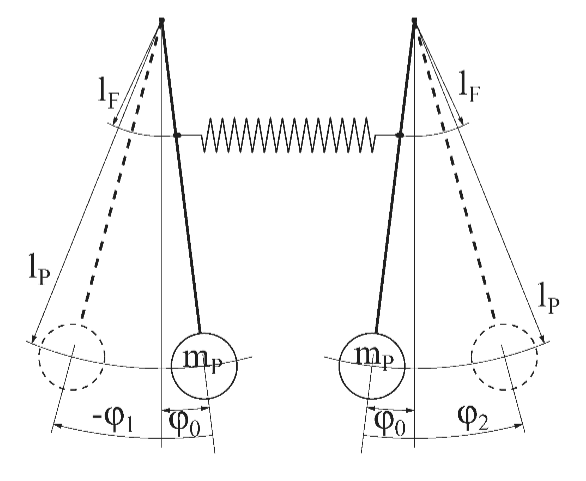
\includegraphics[scale=0.5]{Bilder/Gekoppeltes-Pendel.PNG}
\end{figure}

In diesem Versuch wird der Kopplungsgrad eines gekoppelten Pendels und die Federkonstante der Feder bestimmt, die für die Kopplung verantwortlich ist.
Die Feder erzeugt ein Drehmoment von
\begin{equation*}
M_{F,0}=-D_F \cdot x_0 \cdot l_F
\end{equation*}
welches durch das von der Schwerkraft erzeugte Drehmoment 
\begin{equation*}
M_{S,0}=m \cdot g \cdot l_s \cdot \phi_0
\end{equation*}
kompensiert wird.
So ergibt sich für das gesamte Drehmoment, wenn ein Pendel um $\phi_2$ ausgelenkt wird:
\begin{equation*}
M_2=-m \cdot g \cdot l_s \cdot \phi_2 - D_F \cdot l_F^2 \cdot \phi_2
\end{equation*}
Daraus ergibt sich für die Bewegungsgleichungen der beiden Pendel:
\begin{align*}
\ddot{\phi_1}=-\omega_s^2 \cdot \phi_1 + \Omega^2 \cdot (\phi_2 - \phi_1) \\
\ddot{\phi_2}=-\omega_s^2 \cdot \phi_2 - \Omega^2 \cdot (\phi_2 - \phi_1)
\end{align*}
Dabei sind:
\begin{align*}
\omega_s~und~\omega_{sf}=\sqrt{\omega_s^2+2\Omega^2}
\end{align*}
Lösungen dieses Systems aus gekoppelten Differenzialgleichungen.
Der Kopplungsgrad wird definiert als:
\begin{align}
\kappa =\frac{D_F l_F^2}{mgl_s + D_F l_F^2}= \frac{\omega_{sf}^2-\omega_{s}^2}{\omega_{sf}^2+\omega_s^2}
\end{align}
Um die Federkonstante zu bestimmen, wird $\frac{1}{\kappa}$ gegen $\frac{1}{l_F^2}$ aufgetragen:
\begin{align}
\frac{1}{\kappa}=1+\frac{ml_sg}{D_F}\cdot \frac{1}{l_F^2}
\label{k}\\
\end{align}
Zur Überprüfung wird die Federkonstante auch durch
\begin{align}
m \cdot g = -D_F \cdot x
\label{Hook}
\end{align}
bestimmt.
\subsection{Versuchsaufbau und Durchführung}
%Genaue Beschreibung der verwendeten Aufbauten unter Verwendung von Skizzen oder Photos
%Beschreibung der Messwerterfassungseinstellungen (eingestellte Messzeiten, Messbedingungen,
%Trigger, Anzahl der Messungen) und der Durchführung der Versuche. (max. 1 Seite)
\begin{figure}[H]
\centering
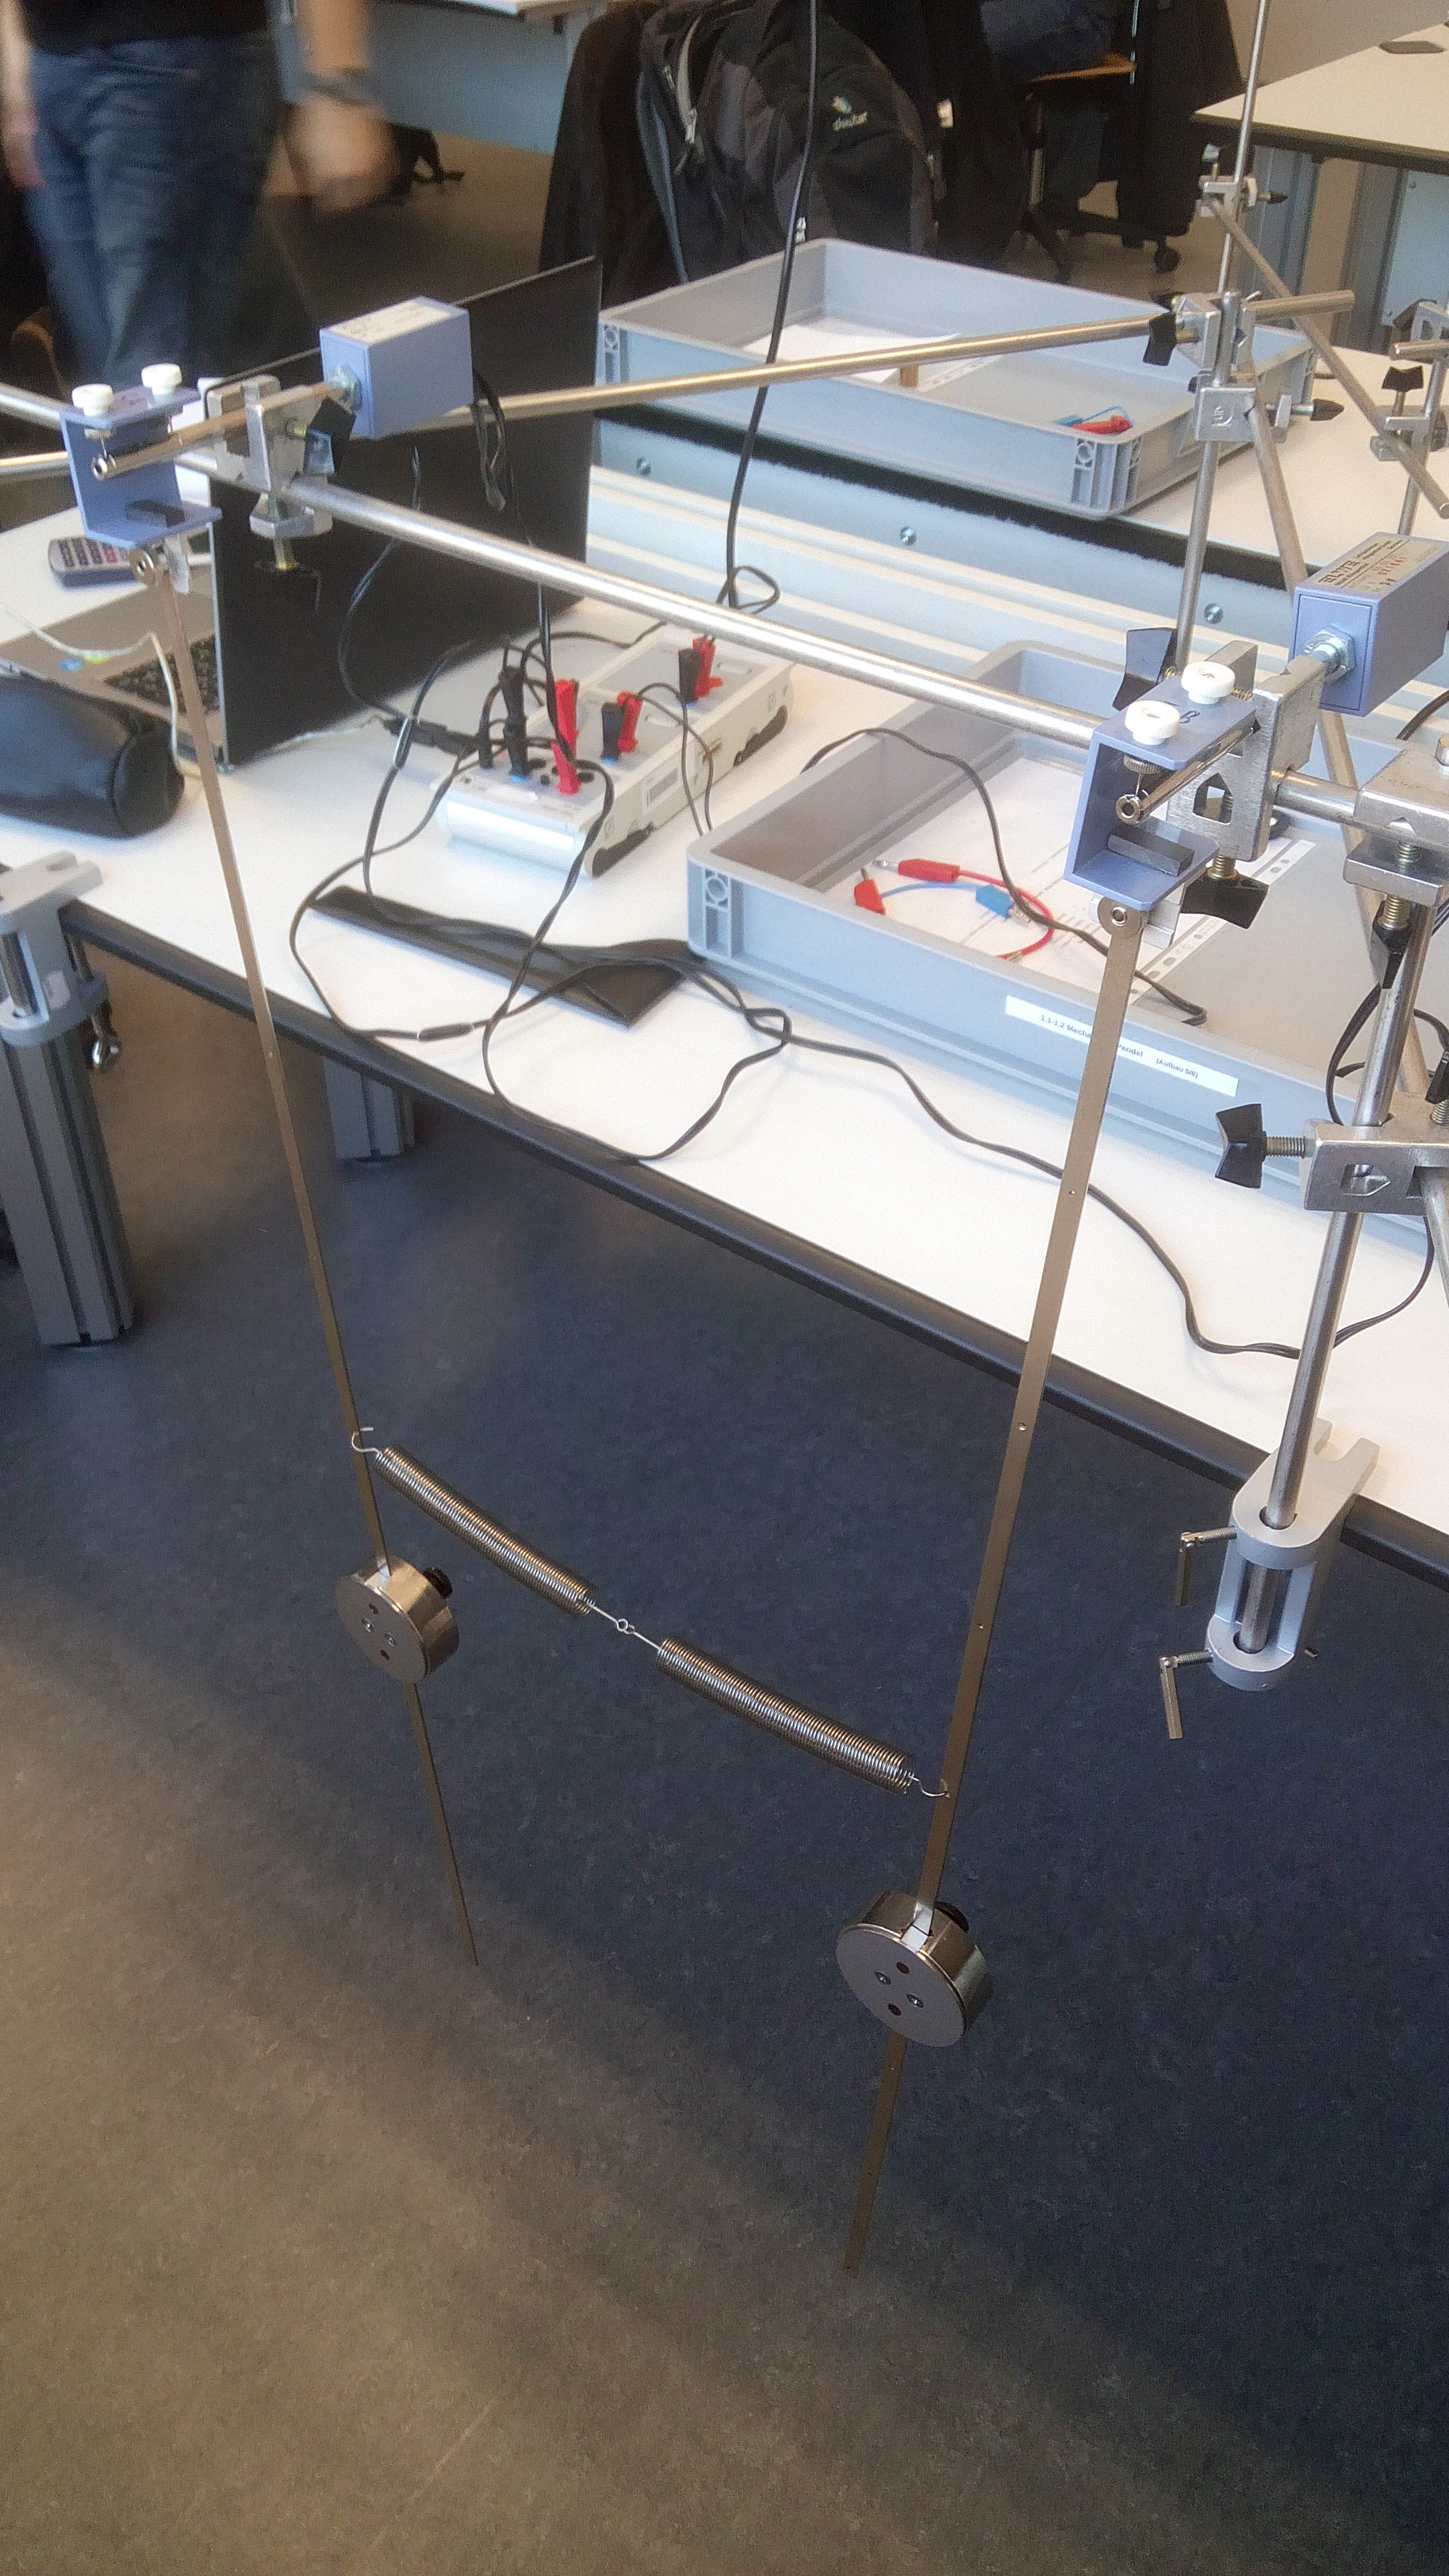
\includegraphics[scale=0.1]{Bilder/Doppelpendel.jpg}
\caption{gekoppeltes Pendel}
\end{figure}
Der Versuchsaufbau des gekoppelten Pendel ist der gleiche wie beim Einzelpendel, bei dem ein zusätzliches, möglichst identisches Pendel verwendet wird. Dieses Pendel wird auf gleicher Höhe im Abstand von ca. 50cm befestigt und mit einer Feder an das andere Pendel gekoppelt. Die Befestigungshöhe der Feder wird dabei variiert, um die Kopplung zu verändern (siehe: \ref{k}). Mittels Linearer Regression lässt sich dann ein Wert für die Federkonstante D bestimmen. \newline
Des Weiteren wurde die Federkonstante aus dem Hook'schen Gesetz (siehe: \ref{Hook}) bestimmt. Dazu haben wir mit verschiedenen Gewichten die Feder belastet und die Auslenkung gegenüber der Ruhelage gemessen.
\subsection{Versuchsauswertung}
\subsubsection{Rohdaten}
\begin{figure}[H]
\centering
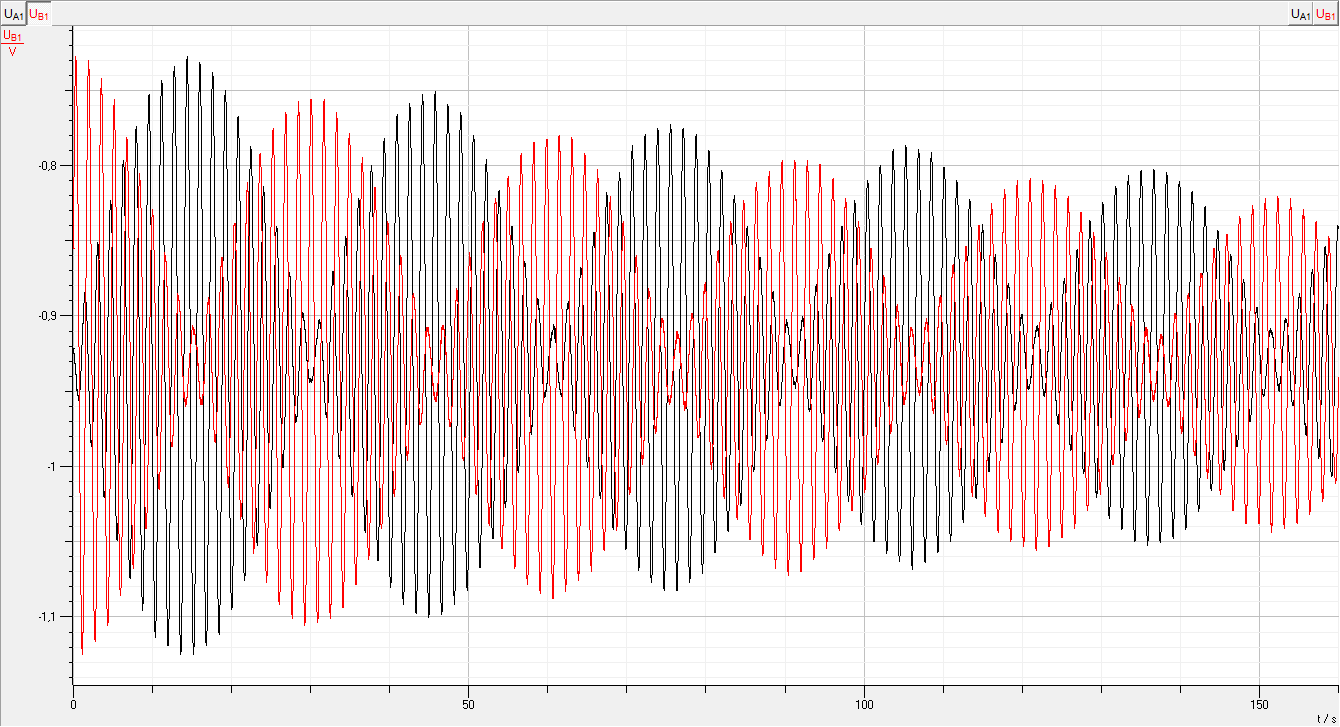
\includegraphics[scale=0.6]{Bilder/Schwebung.png}
\caption{Schwebung Loch 2}
\end{figure}
\begin{figure}[H]
\centering
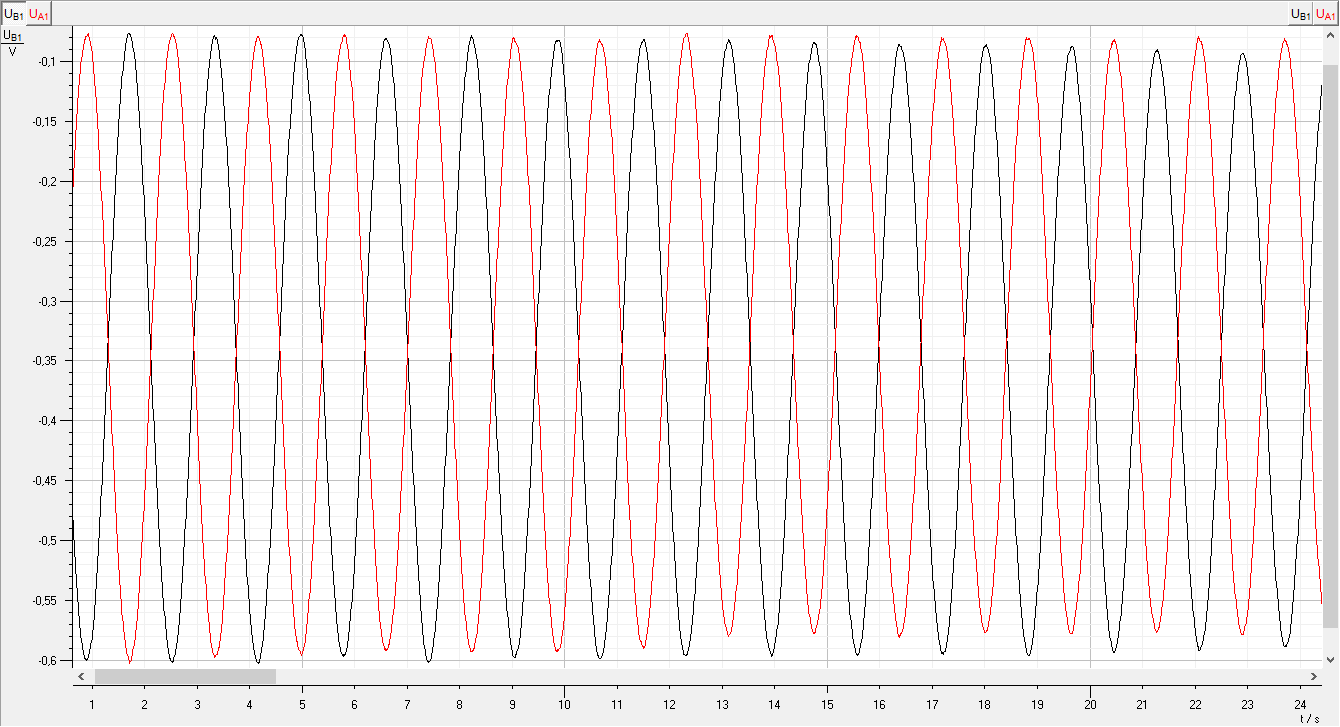
\includegraphics[scale=0.6]{Bilder/Gegensinnig.png}
\caption{Gegensinnige Auslenkung}
\end{figure}
\begin{figure}[H]
\centering
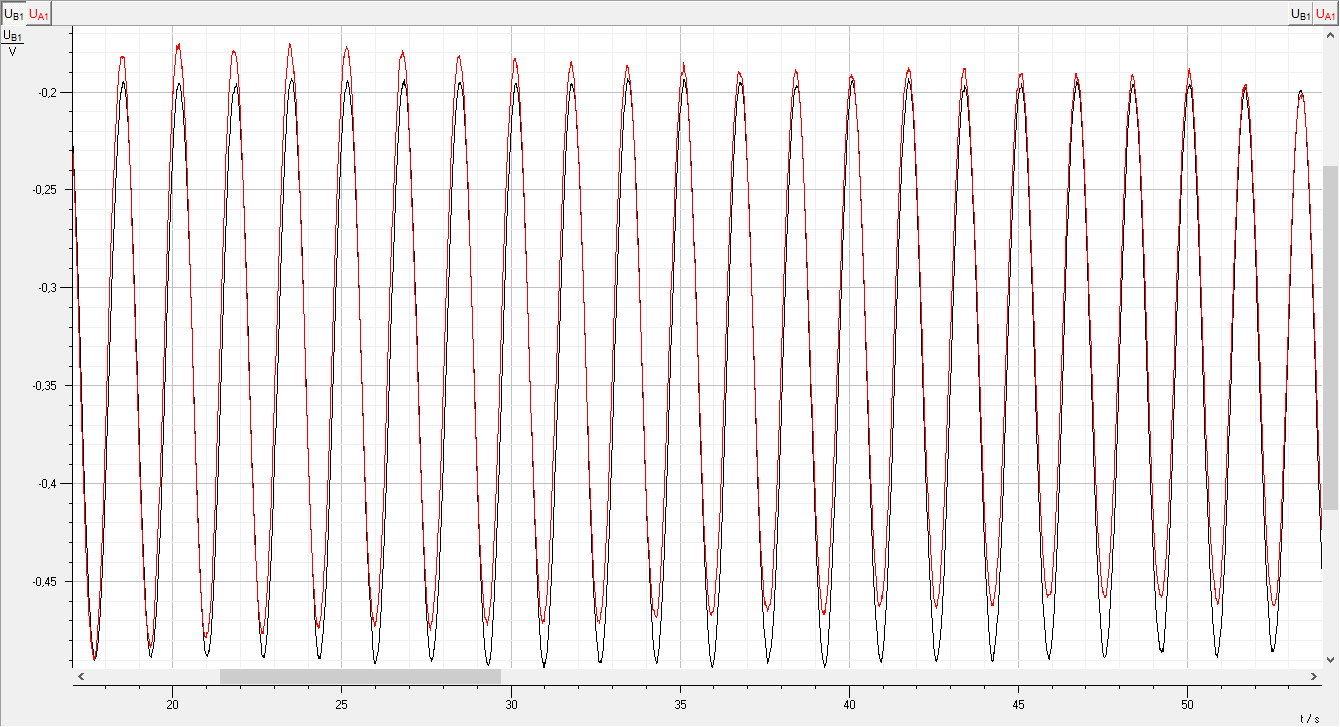
\includegraphics[scale=0.5]{Bilder/Gleichsinnig.png}
\caption{Gleichsinnige Auslenkung}
\end{figure}
\textbf{Daten zur Berechnung von D aus Gleichung (\ref{Hook}):}\newline
Die Ablesefehler wurden bei den Längenmessungen zu $\sigma_x=0.1cm$ bestimmt.\newline
Auslenkung: $x=x_{gemessen}-x_0$ \newline
Ruhelage der Feder Gruppe 1: $x_0=21.6cm$
\begin{table}[H]\centering
\caption{Daten Hook Gruppe 1}
\begin{tabular}{c|c|c|c}
Auslenkung in cm & Fehler in cm & angehängte Masse in g & Fehler der Waage in g\\ 
\hline
$x_1=11.3$& $\sigma_{x_1}=0.1$& $m_1=60$& $\sigma_{m_1}=0.1$\\ 
$x_2=18.7$& $\sigma_{x_2}=0.1$& $m_2=100$& $\sigma_{m_2}=0.1$\\
$x_3=14.9$& $\sigma_{x_3}=0.1$& $m_3=80$& $\sigma_{m_3}=0.1$\\
\end{tabular} 
\end{table}
Ruhelage der Feder Gruppe 2: $x_0=22.8cm$
\begin{table}[H]\centering
\caption{Daten Hook Gruppe 2}
\begin{tabular}{c|c|c|c}
Auslenkung in cm & Fehler in cm & angehängte Masse in g & Fehler der Waage in g\\ 
\hline
$x_1=22.2$& $\sigma_{x_1}=0.1$& $m_1=120.5$& $\sigma_{m_1}=0.1$\\ 
$x_2=18.3$& $\sigma_{x_2}=0.1$& $m_2=103$& $\sigma_{m_2}=0.1$\\
$x_3=8.9$& $\sigma_{x_3}=0.1$& $m_3=50.3$& $\sigma_{m_3}=0.1$\\
$x_4=3.3$& $\sigma_{x_4}=0.1$& $m_4=20$& $\sigma_{m_4}=0.1$\\
\end{tabular} 
\end{table}
\begin{table}[H]\centering
\caption{Löcher mit ihren Abständen vom Aufhängepunkt}
\begin{tabular}{c|c|c|c}
Löcher &Gruppe 1&Gruppe 2\\ 
\hline
$1.$& $15.8cm$& $16.4cm$\\ 
$2.$& $27.8cm$& $28.5cm$\\
$3.$& $40.4cm$& $41cm$\\
$4.$& $52.9cm$& $53.5cm$\\
$6.$& $77.6cm$& $78.5cm$\\ 
$7.$& $89.6cm$& $90.5cm$\\
$8.$& $101.6cm$& $102.6cm$\\
\end{tabular} 
\end{table}
\newpage
\subsubsection{Transformation der Rohdaten/Analyse}
Aus der Schwebung des Doppelpendels ergeben sich mit Fast-Fourier-Transformation $\omega_s$ und $\omega_{sf}$ durch $\omega=2\pi f$:
\begin{figure}[H]
\centering
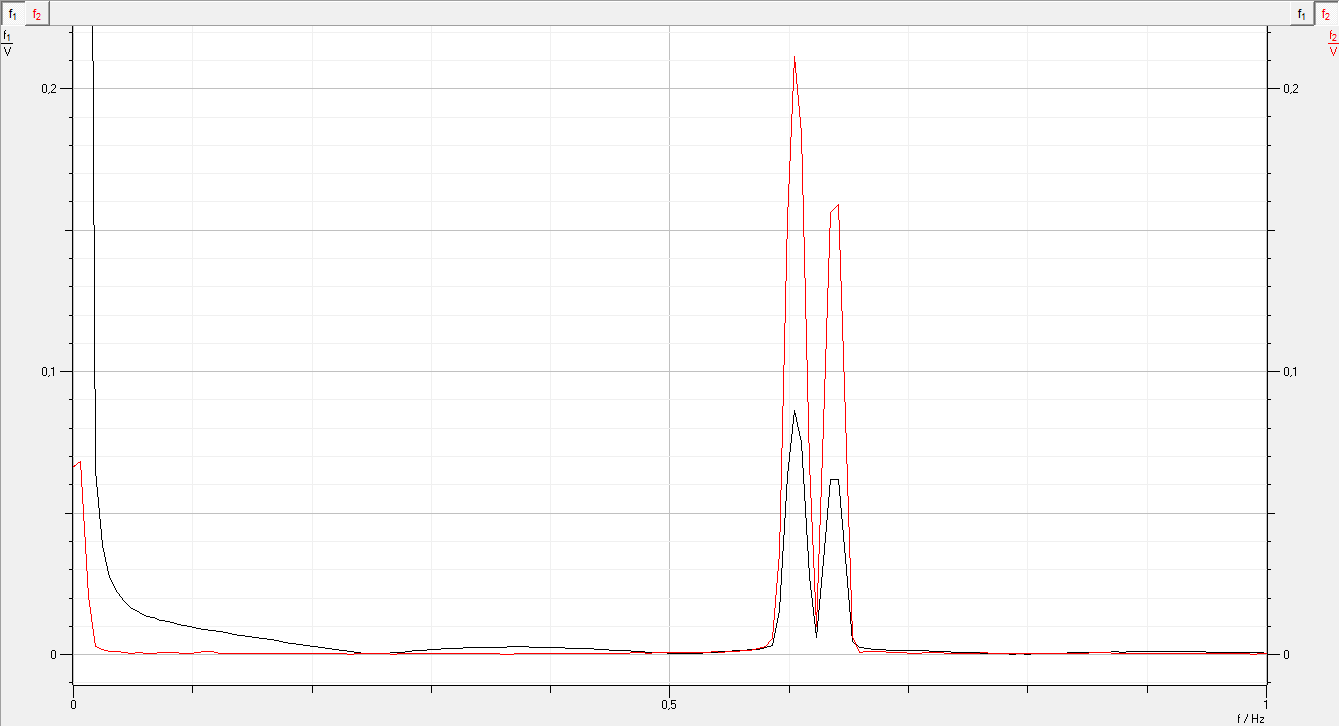
\includegraphics[scale=0.6]{Bilder/FFT-Schwebung.png}
\caption{FFT-Schwebung}
\end{figure}
$~$ \newline
Die geringere Frequenz $f_s$ sieht man bei der gleichsinnigen und die größere Frequenz $f_{sf}$ bei der gegensinningen Auslenkung.
\newline
Für die verschiedenen Positionen der Feder wurde das 5. Loch vom Pendelkörper blockiert und die Kopplung des ersten Lochs war so gering, dass wir nur eine Frequenz ermitteln konnten, so dass wir diese Werte im Folgenden nicht mehr betrachten.
Für die anderen Positionen wurde jeweils per FFT die Frequenzen mit ihren Ablesefehlern bestimmt. Der Ablesefehler wurde durch mehrfache Peakschwerpunktbestimmung ermittelt.
\begin{figure}[H]
\centering
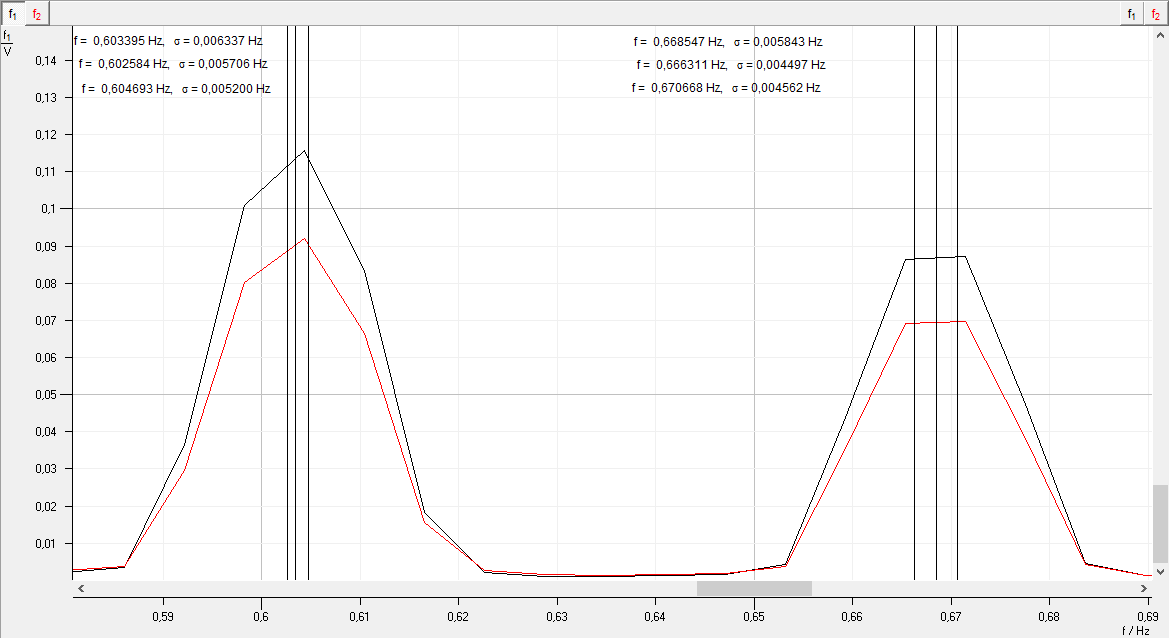
\includegraphics[scale=0.42]{Bilder/fft_Fehlermessung.png}
\caption{Peakschwerpunktsbestimmung}
\end{figure}

\begin{figure}[H]
\centering
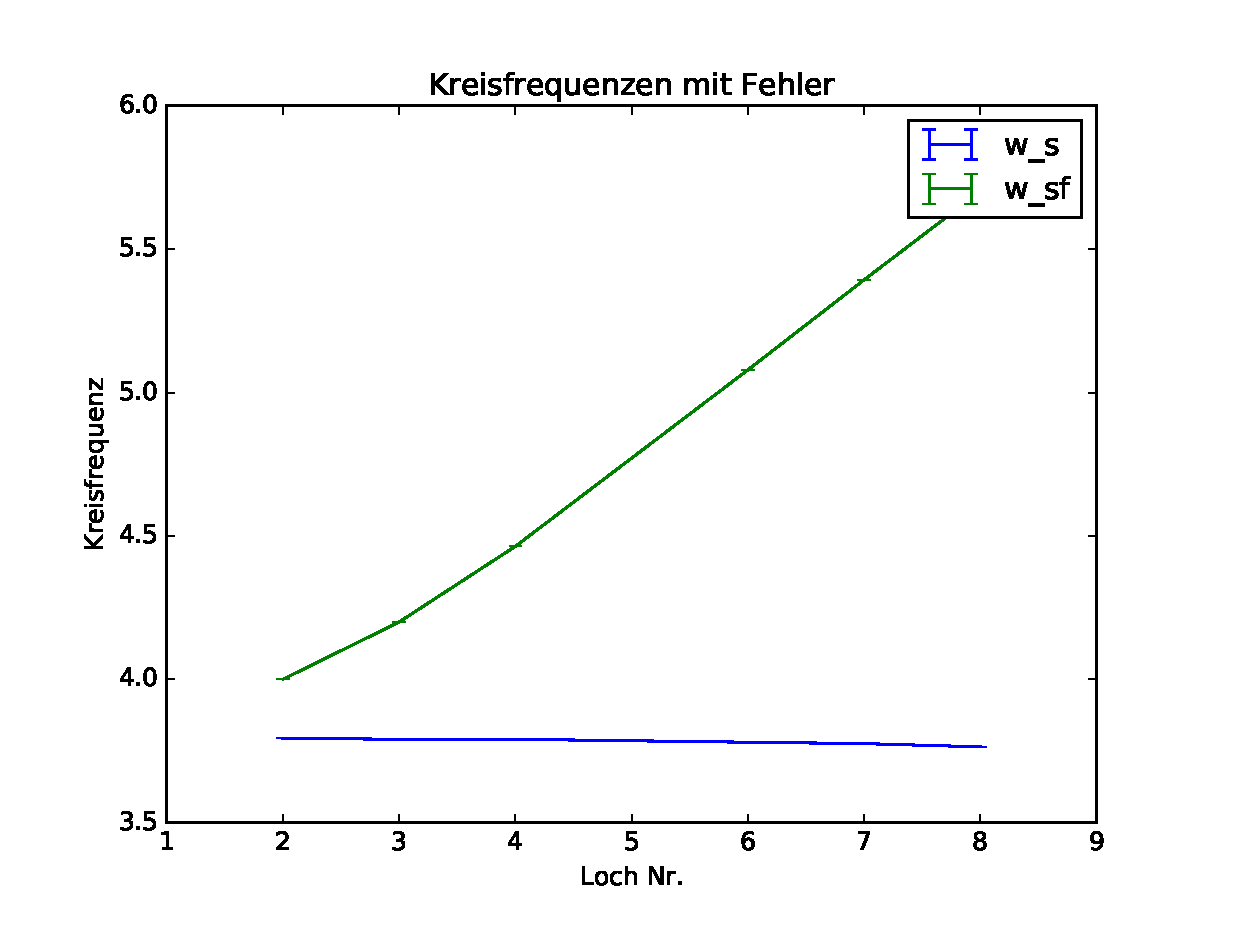
\includegraphics[scale=0.7]{Bilder/Kreisfrequenzen_fuer_Kappa.eps}
\caption{Loch/Frequenzen}
\end{figure}
Aus diesen Frequenzen wurde anschließend $\kappa$ durch Gleichung (\ref{k}) bestimmt.
\newline
Nun wurde $\frac{1}{\kappa}$ gegen $\frac{1}{l_F^2}$ aufgetragen um aus der Steigung die Federkonstante bestimmen zu können.
\begin{figure}[H]
\centering
\caption{}
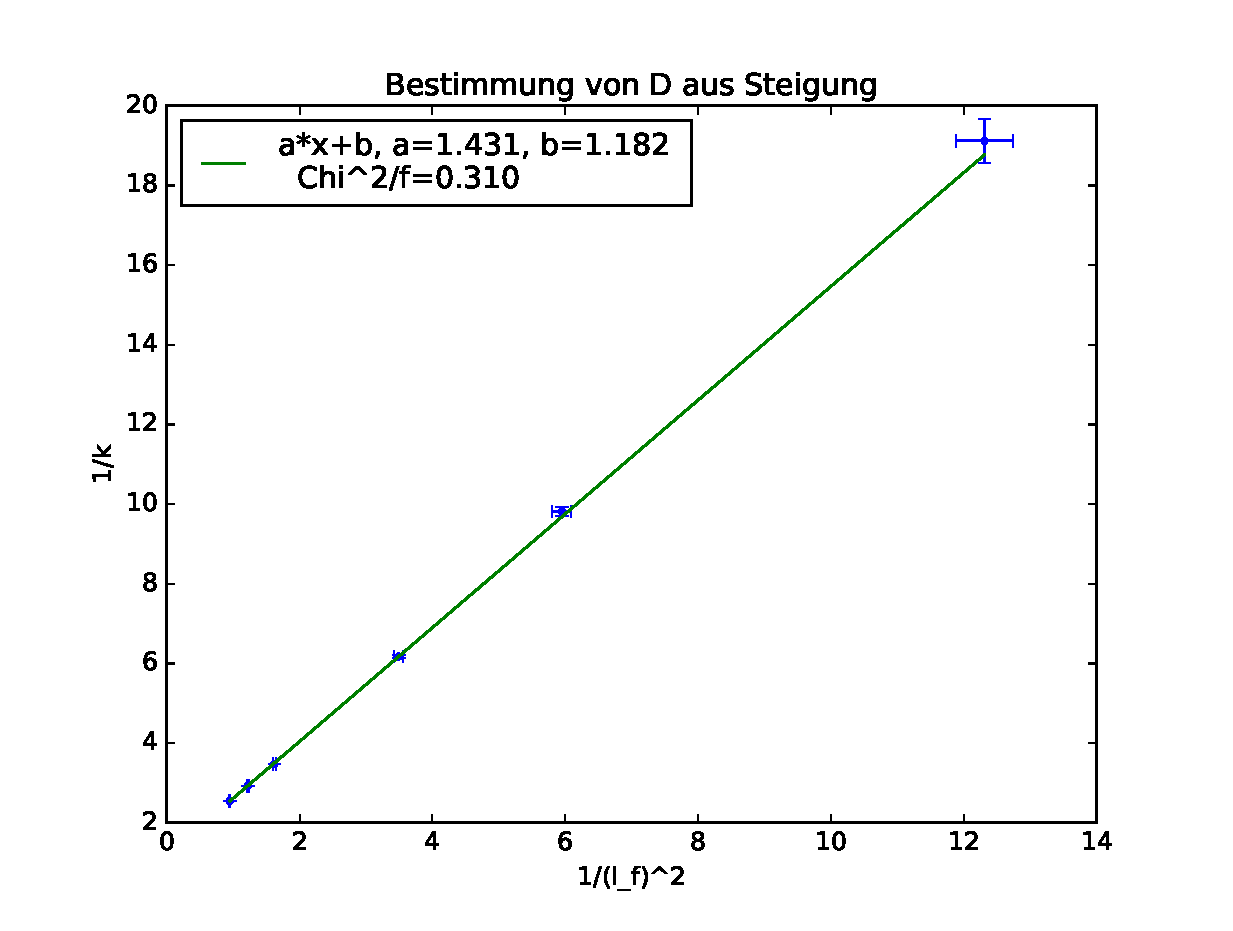
\includegraphics[scale=0.7]{Bilder/Bestimmung_D_linreg.eps}
\end{figure}
Die gesuchte Federkonstante D ergibt sich dann aus:
\begin{align}
D_F=m \cdot l_s \cdot \frac{g}{a}\\
\sigma_{D_F}=m \cdot \sqrt{(g\cdot \frac{\sigma_{l_s}}{a})^2+(g\cdot l_s \cdot \frac{\sigma_a}{a^2})^2+(l_s \cdot \frac{\sigma_g}{a})^2}
\end{align}
Wobei hier g mit entsprechenden Fehlern aus dem Einzelpendelversuch benutzt wurde.
\begin{table}[H]\centering
\caption{$D_F$ aus Doppelpendel}
\begin{tabular}{c|c}
Gruppe 1 & Gruppe 2\\ 
\hline
$D_F=4.9636\frac{1}{m}$& $D_F=4.8491 \frac{1}{m}$\\ 
$\sigma_{D_F}=0.1622 \frac{1}{m}$& $\sigma_{D_F}=0.0609 \frac{1}{m}$\\
\end{tabular} 
\end{table}
An der zugehörigen, um 0 streuenden Residuenverteilung sieht man, dass die Anpassung der Geraden uns unsere Werte sinnvoll war:
\begin{figure}[H]
\caption{}
\centering
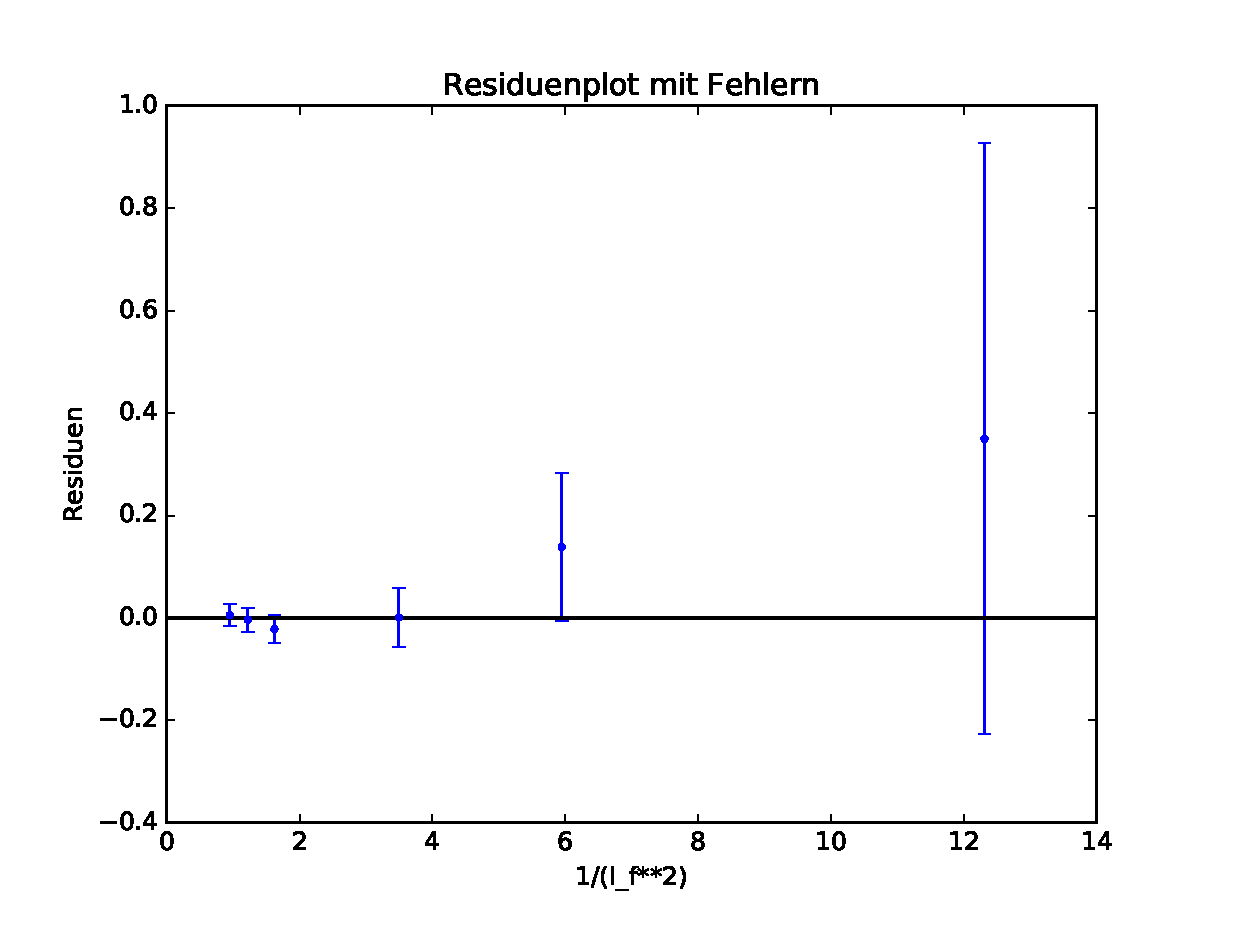
\includegraphics[scale=0.8]{Bilder/Bestimmung_D_Residuen.eps}
\end{figure}

Nun wurde zum Vergleich die Federkonstante noch einmal über das Hook'sche Gesetz (siehe: \ref{Hook}) bestimmt: 
\begin{figure}[H]
\caption{}
\centering
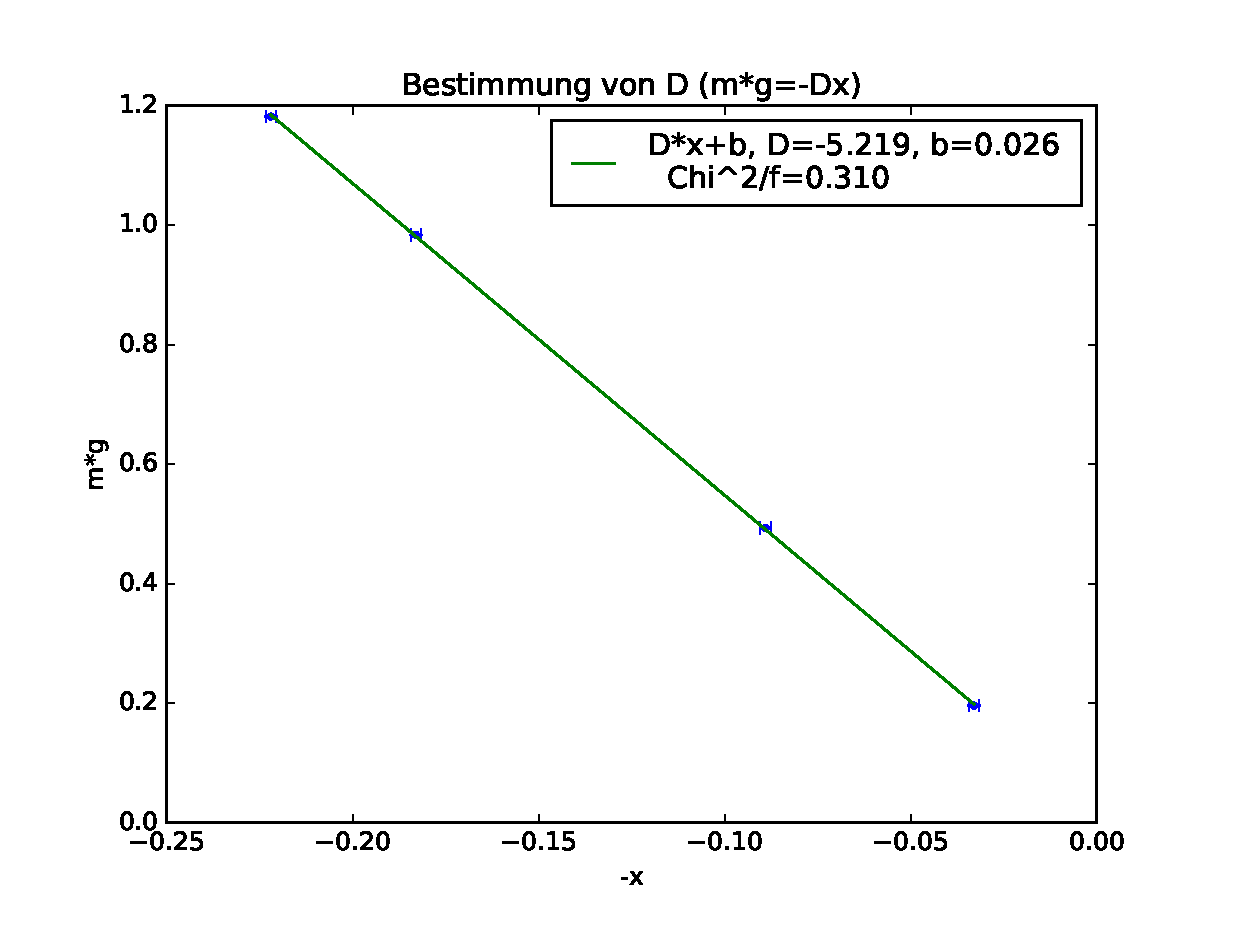
\includegraphics[scale=0.8]{Bilder/Hook_linreg.eps}
\end{figure}
\begin{equation*}
D_F=-\frac{m\cdot g}{x_0}
\end{equation*}
\begin{table}[H]\centering
\caption{$D_F$ aus Hook}
\begin{tabular}{c|c}
Gruppe 1 & Gruppe 2\\ 
\hline
$D_F=5.2671 \frac{1}{m}$& $D_F=5.219 \frac{1}{m}$\\ 
$\sigma_{D_F}=0.102 \frac{1}{m}$& $\sigma_{D_F}=0.0246 \frac{1}{m}$\\
\end{tabular} 
\end{table}
\begin{figure}[H]
\caption{}
\centering
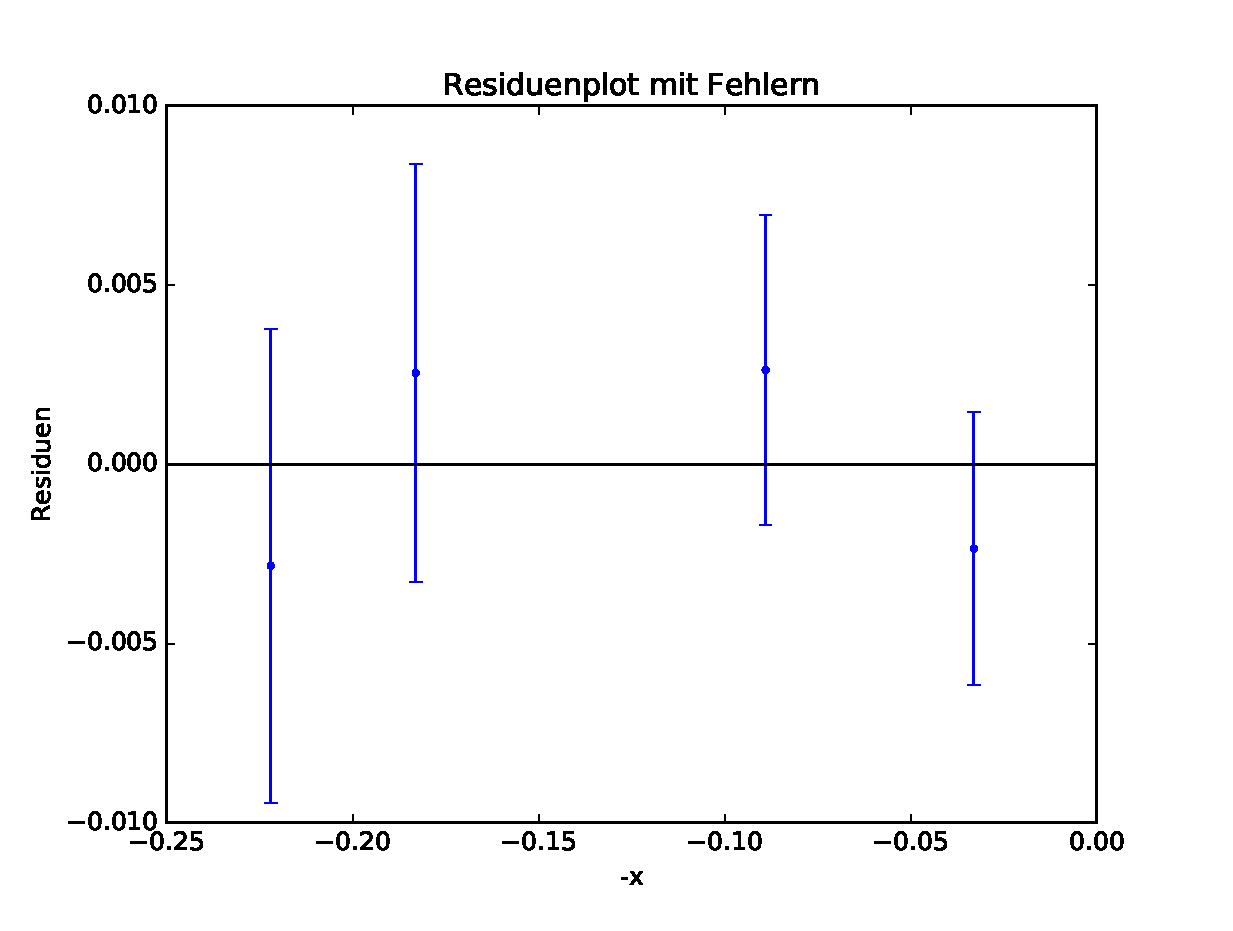
\includegraphics[scale=0.8]{Bilder/Hook_residuen.eps}
\end{figure}

\subsubsection{Fazit}
%Diskussion der Ergebnisse und Vergleich der erzielten Ergebnisse mit theoretischen Vorhersagen.
%(1 Seite)
Unsere Ergebnisse bei der Berechnung der Federkonstante stimmen mit ihren Fehlern nicht ganz überein. Bei Gruppe 2 gibt es sogar deutliche Abweichungen. Nach langer Diskussion erklären wir uns dies durch die Näherung unseres Pendels an einen homogenen zylindrischen Pendelkörper mit masseloser Pendelstange, die durch die angepasste Frequenz an die Pendelstange ohne Pendelkörper gegeben wird. Gruppe 2 hat hier eine Anpassung mit einem drei mal größeren Fehler auf die Frequenz (siehe: \ref{Abscheichungen der Frequenzen}). Diese Ungenauigkeit in der Näherung zieht sich als systematischer Fehler durch die gesamte Rechnung. Dass wir nur statistische Fehler betrachtet haben, die Systematik aber einen nicht geringen Anteil am Fehler hat, erklärt unsere Abweichung der Ergebnisse aus dem Doppelpendel und der Hook'schen Federmessung.
\newline
Bei den Linearen Regressionen kann man erkennen, dass die Geraden alle Fehlerkästen schneiden.
Auch die Residuenplots entsprechen unseren Erwartungen, es sind keine Systematiken erkennbar. Somit sind unsere statistischen Fehler im Rahmen unserer Erwartungen.
\end{document}
